\ChapterImageStar[cap:disenio]{Diseño de la solución}{./images/fondo.png}\label{cap:disenio}
\mbox{}\\

El presente capítulo tiene como objetivo fundamental traducir la decisión estratégica —la implementación de los Universos Grid y Parallel— en un diseño técnico y estratégico concreto y ejecutable. Aquí se especifica la arquitectura de la solución, detallando los componentes de HTCondor que serán configurados o modificados, los flujos de trabajo establecidos para cada universo y los criterios de interoperabilidad con el Universo Vanilla preexistente. Este diseño busca establecer las bases técnicas y metodológicas para la fase de implementación, propendiendo por la robustez, escalabilidad e integridad de la infraestructura de computación distribuida resultante. Además, busca ayudar al Grupo \GRID con el cumplimiento de sus objetivos estratégicos y el cierre de la brecha identificada en la caracterización.

\section{Definición de estrategia}
La definición de la estrategia de diseño se fundamenta en una filosofía de desarrollo guiado por pruebas (\TDD), que es una disciplina de diseño y programación donde cada línea de código está escrita en respuesta a una prueba que el programador escribe justo antes de escribir el código \parencite{4163024}. Antes de especificar los componentes arquitectónicos, se establece un conjunto de casos de prueba estructurados que definen de manera formal y verificable el comportamiento esperado de los Universos \textit{Grid} y \textit{Parallel}. Estos casos, que funcionan como criterios de aceptación guiarán de manera iterativa el diseño de la solución, asegurando que cada decisión de implementación esté directamente alineada con la validación funcional del sistema.

Por último, se considera necesario establecer un nombre para el sistema. Esto con el fin de dar mayor claridad al lector y hacer más visibles los momentos en los que se habla del sistema resultado de este proyecto. Se opta por el "Grid App" haciendo referencia al Grupo \GRID, que es el sujeto nuclear de este proyecto; al Universo Grid, que es uno de los Universos que se decidió implementar para este proyecto de aplicación después de la toma de decisiones estructurada mediante el análisis \DAR y el modelo computacional Grid que es básicamente una infraestructura que provee gran capacidad computacional a un sistema distribuido haciendo uso de recursos geográficamente distribuidos \parencite{8974490}.

\section{Casos de prueba}

\subsection{Definición de requisitos}
\noindent
Para iniciar con la definición de casos de prueba, se establecen los requisitos que debe cumplir \textit{Grid App} que están fundamentados en el análisis preliminar hecho anteriormente, principalmente en la descripción de la oportunidad para el Grupo \GRID.

\subsubsection{Requisitos funcionales}
\noindent
Según \textcite{159342} un requisito funcional especifica una función que el sistema o que un componente del sistema es capaz de hacer. A continuación se definen los requisitos funcionales para \textit{Grid App}.
\begin{table}[H]
	\centering
	\sffamily\scriptsize
	\setlength{\tabcolsep}{4pt}
	\renewcommand{\arraystretch}{1.3}
	\caption{Requisitos funcionales para \textit{Grid App}}
	\label{table:requisitosFuncionales}
	\begin{tabular}{|p{0.1\textwidth}|p{0.2\textwidth}|p{0.7\textwidth}|}
		\toprule
		\textbf{ID}                              & \textbf{Título}                               & \textbf{Descripción} \\
		\midrule
		RF1 & Soporte para Universos adicionales & El sistema debe permitir la ejecución de trabajos en al menos dos Universos adicionales a Vanilla (Grid y Parallel) \\
		\midrule
		RF2 & Orquestación de múltiples clústeres & El sistema debe permitir enviar trabajos hacia diferentes clústeres (Parallel, Vanilla) a través del Universo Grid. \\
		\midrule
		RF3 & Selección de destino & El sistema debe permitir que el usuario especifique el clúster de destino. \\
		\midrule
		RF4 & Monitoreo de trabajos & El sistema debe permitir el monitoreo de los trabajos enviados a los clústeres, mostrando su estado al usuario. \\
		\midrule
		RF5 & Ejecución MPI en Parallel & Un clúster debe soportar ejecución de trabajos basados en MPI en múltiples nodos (≥ N nodos configurados). \\
		\midrule
		RF6 & Redirección Grid-Parallel & El Grid Manager debe aceptar trabajos enviados al Universo Grid y, si la naturaleza del trabajo es paralelo, redirigirlos correctamente al Universo Parallel. \\
        \midrule
		RF7 & Redirección Grid-Vanilla & El Grid Manager debe aceptar trabajos enviados al Universo Grid y, si la naturaleza del trabajo es distribuido, redirigirlos correctamente al Universo Vanilla. \\
        \midrule
		RF8 & Registro centralizado de errores & El Grid Manager debe centralizar \textit{logs} de fallos de ejecución provenientes de cada clúster. \\
		\bottomrule
	\end{tabular}
\end{table}

\subsubsection{Requisitos no-funcionales}
\noindent
Según \textcite{4384163} un requisito no-funcional es un atributo o una restricción de un sistema. A continuación se definen los requisitos no-funcionales para \textit{Grid App}.
\begin{table}[H]
	\centering
	\sffamily\scriptsize
	\setlength{\tabcolsep}{4pt}
	\renewcommand{\arraystretch}{1.3}
	\caption{Requisitos no-funcionales para \textit{Grid App}}
	\label{table:requisitosNoFuncionales}
	\begin{tabular}{|p{0.1\textwidth}|p{0.2\textwidth}|p{0.7\textwidth}|}
		\toprule
		\textbf{ID}                              & \textbf{Título}                               & \textbf{Descripción} \\
		\midrule
		RNF1 & Transparencia de uso & El usuario no debe preocuparse por las configuraciones internas de cada clúster; el Grid Manager abstrae el destino mediante una interfaz más amigable. \\
		\midrule
		RNF2 & Usabilidad & La configuración de los nuevos Universos debe estar documentada y ser accesible mediante manual de despliegue para los usuarios del Grupo GRID. \\
		\midrule
		RNF3 & Disponibilidad & En caso de que un clúster esté inactivo, el Grid Manager debe registrar el error y permitir redirección a otro clúster disponible si el Universo es compatible. \\
		\bottomrule
	\end{tabular}
\end{table}

\subsection{Pruebas}
\noindent
Para esta sección, se definen las pruebas y los pasos de cada prueba a ejecutar 

\section{Modelado del sistema en Archimate}
ArchiMate es un lenguaje de modelado estandarizado por~\textit{The Open Group} que permite representar de manera estructurada y clara las diferentes capas de una arquitectura empresarial: negocio, aplicación y tecnología. Su propósito es brindar una visión integrada que facilite la comunicación entre los distintos actores de un proyecto y que muestre cómo los procesos de negocio, los sistemas de información y la infraestructura tecnológica se relacionan entre sí.
En particular, ArchiMate se organiza en vistas que permiten enfocarse en aspectos específicos: la vista de negocio describe los procesos y actores implicados, la vista de aplicación se centra en los sistemas de software que apoyan esos procesos, y la vista de tecnología aborda la infraestructura que soporta todo el ecosistema. Gracias a este enfoque por capas, los diagramas ayudan a identificar dependencias, puntos de optimización y la coherencia general de la solución arquitectónica.

\subsection{Vista de negocio}


\subsection{Vista de aplicación}
%\begin{figure}[H]
    \centering
    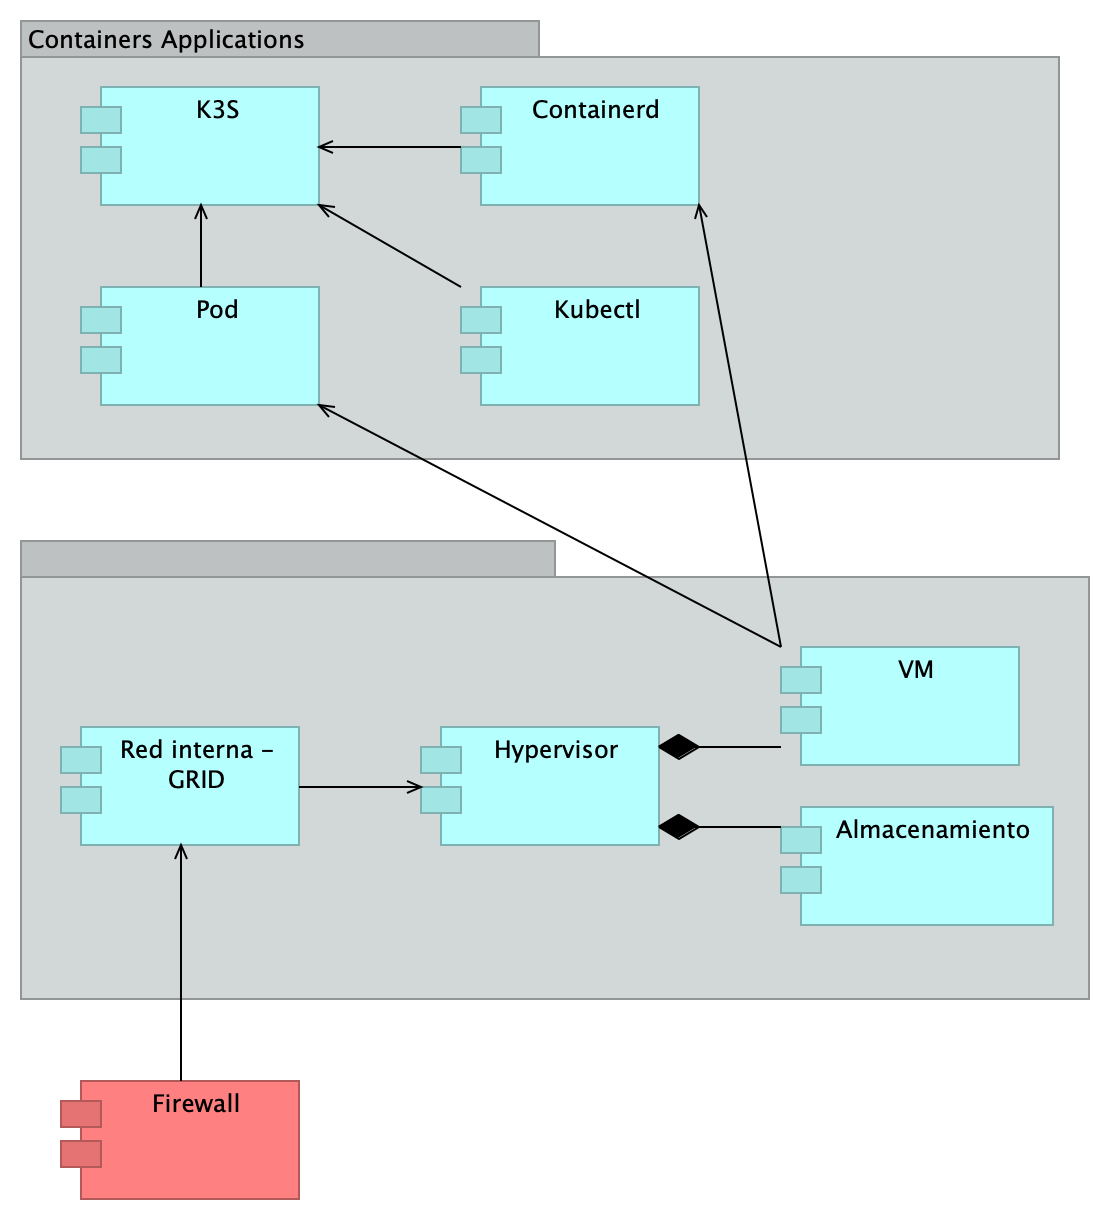
\includegraphics[width=\textwidth]{tablas-images/cp6/Application-Cooperation-View.png}
    \caption{Vista de Cooperación de Aplicaciones}
\end{figure}
\begin{figure}[H]
    \centering
    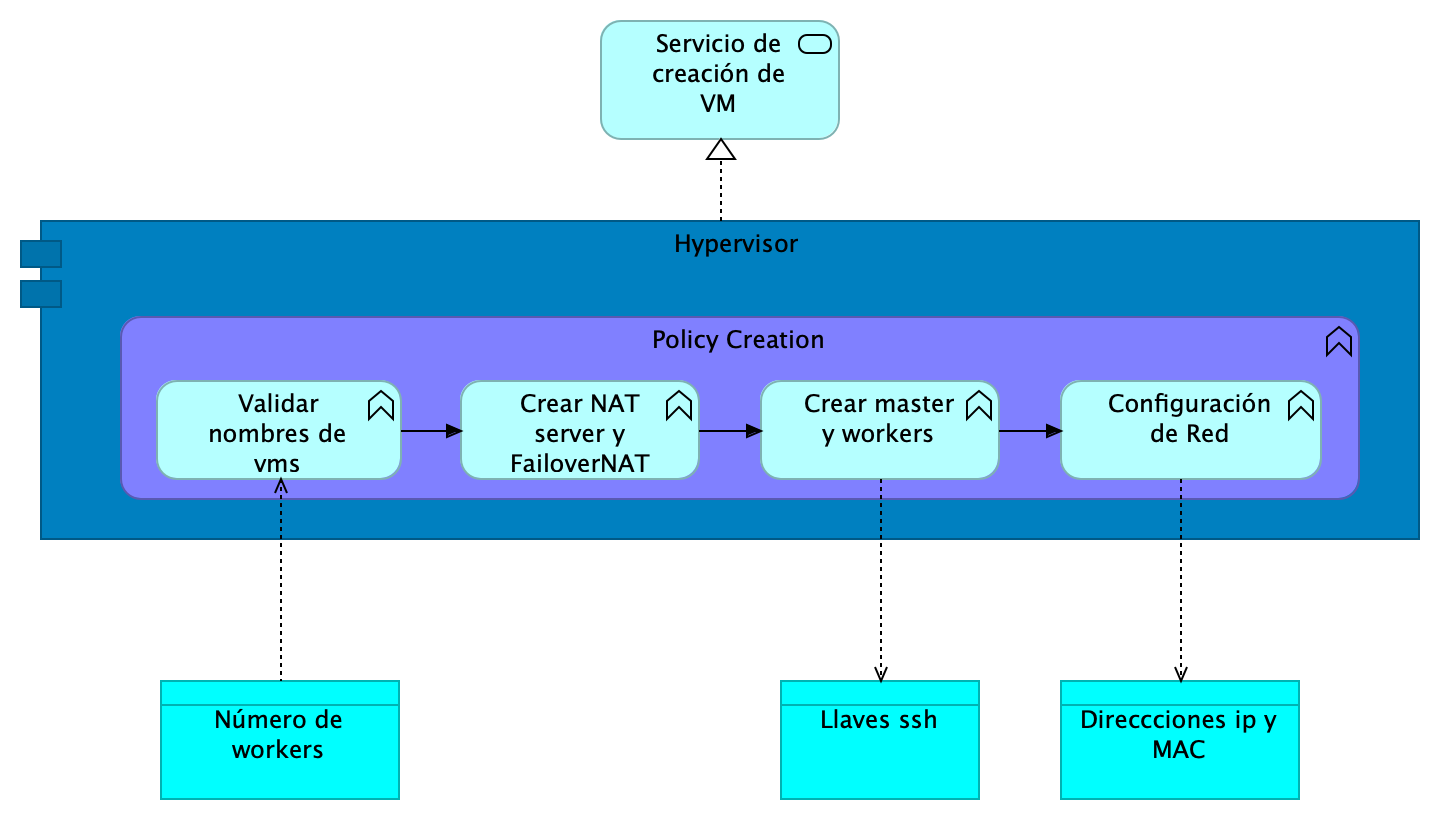
\includegraphics[width=\textwidth]{tablas-images/cp6/Application-Behaviour-view.png}
    \caption{Vista de Comportamiento de Aplicaciones}
\end{figure}
\begin{figure}[H]
    \centering
    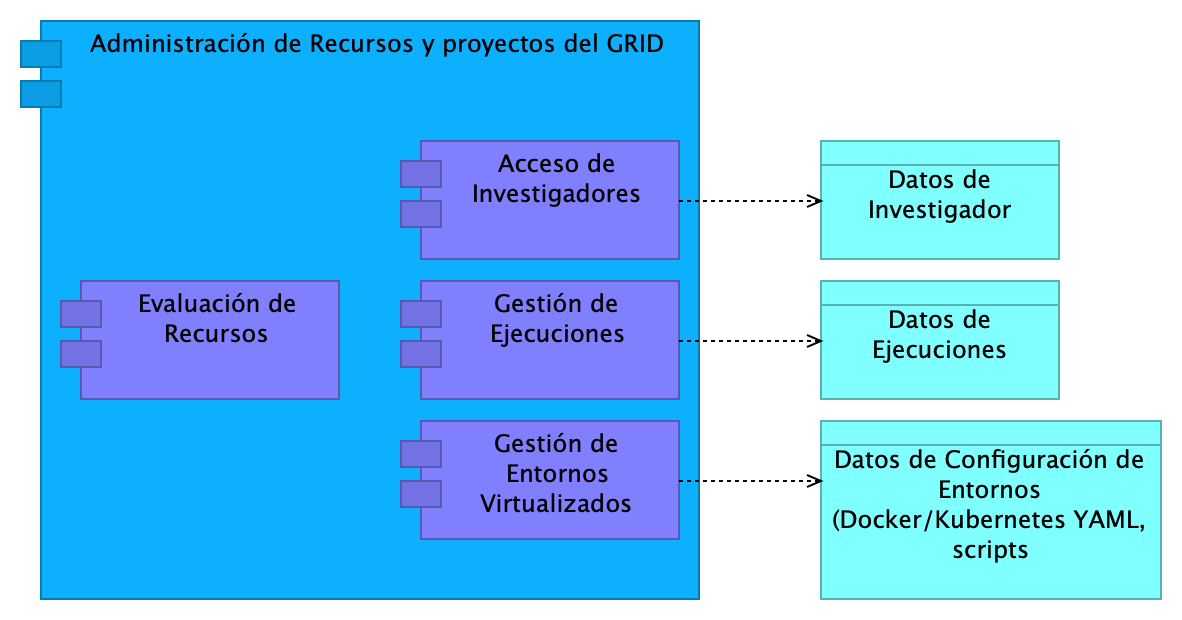
\includegraphics[width=\textwidth]{tablas-images/cp6/Application-Structure-View.png}
    \caption{Vista de Estructura de Aplicaciones}
\end{figure}

\subsection{Vista de tecnología}
%\begin{figure}[H]
    \centering
    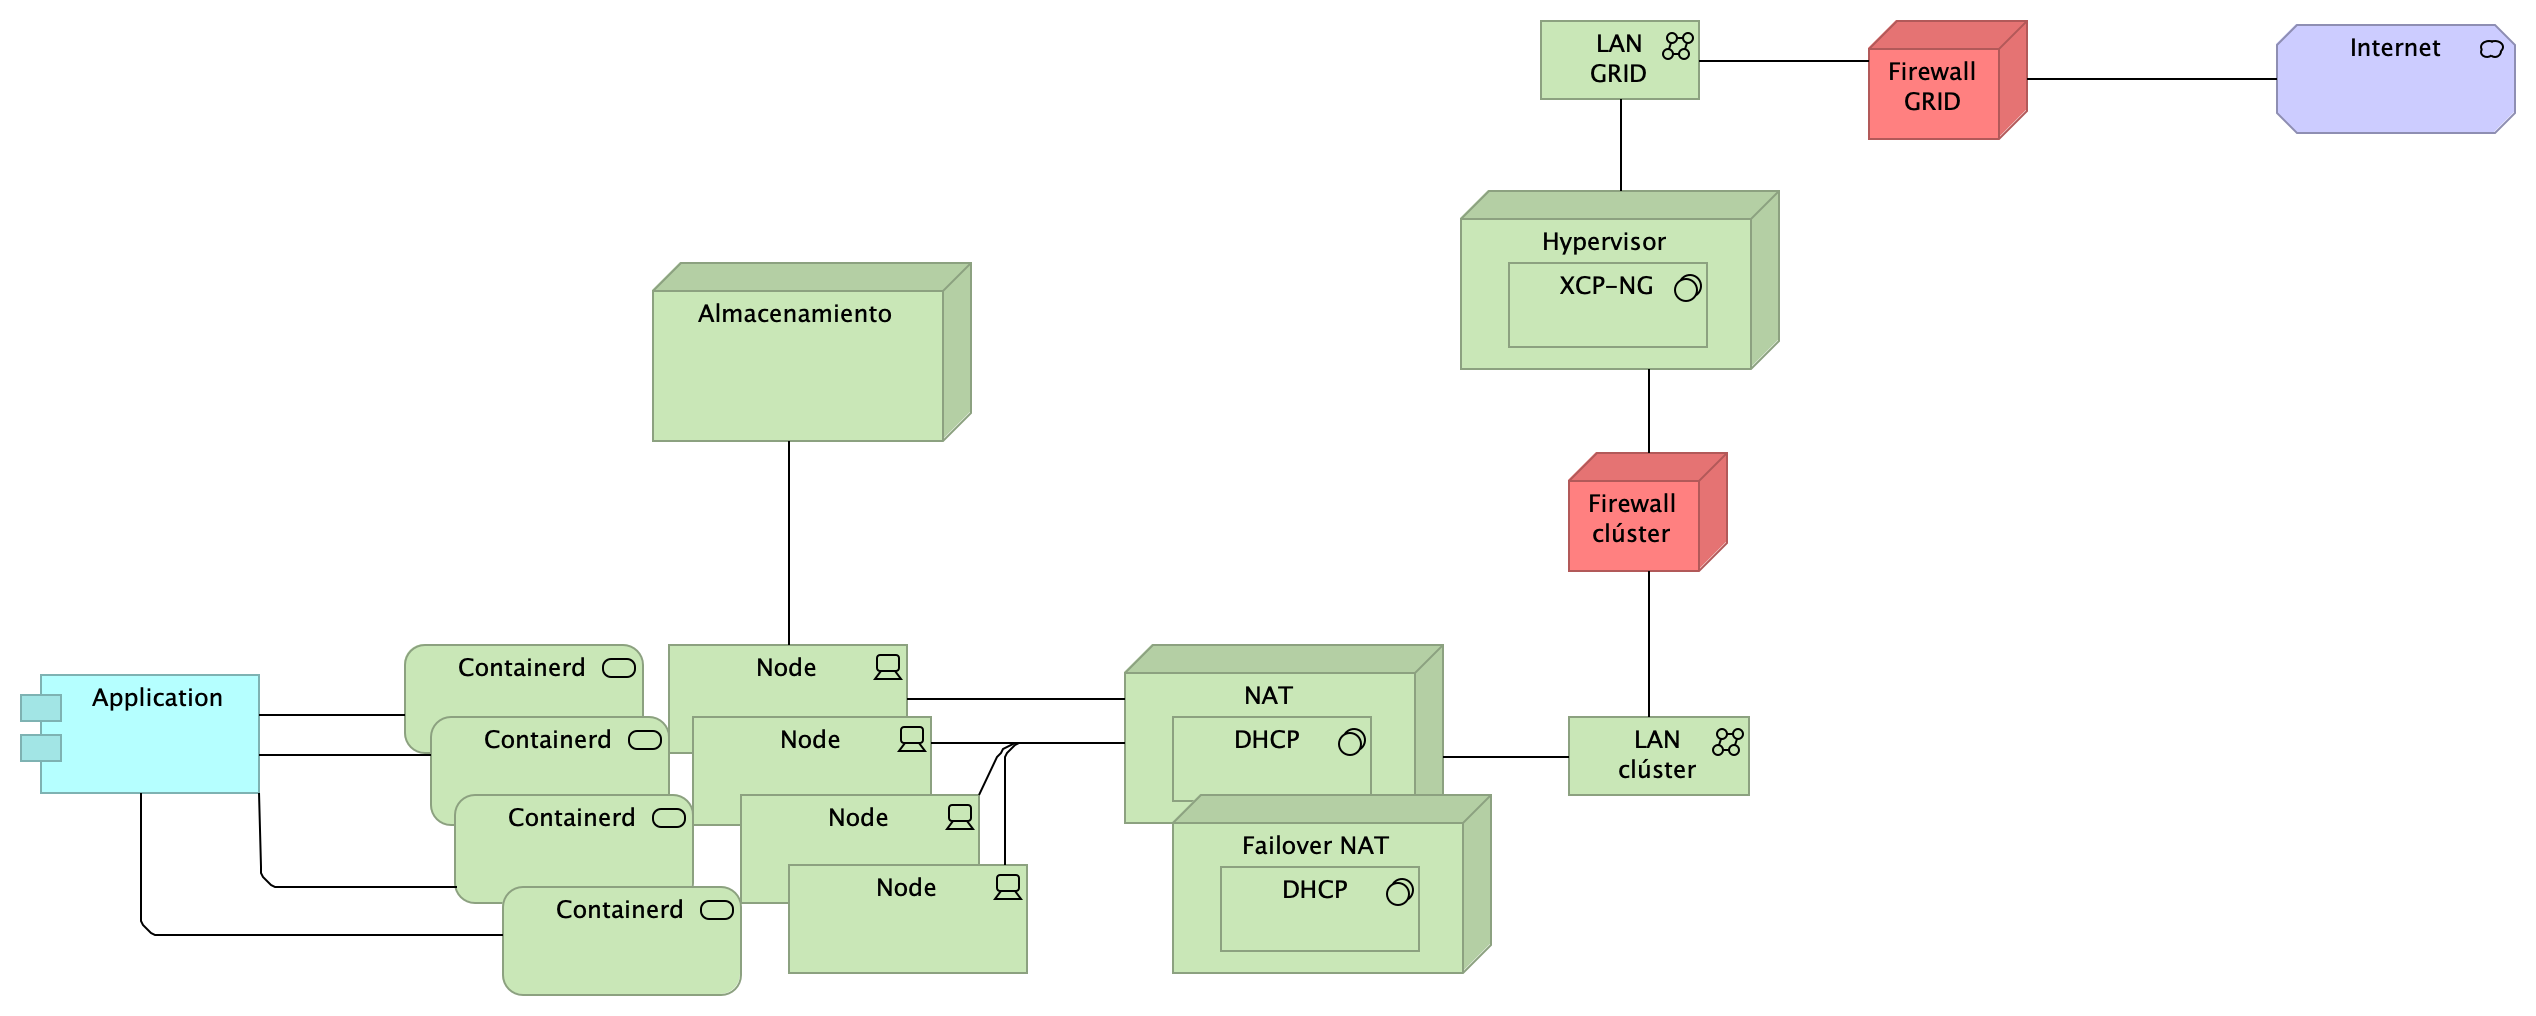
\includegraphics[width=\textwidth]{tablas-images/cp6/Implementation-and-Installation-View.png}
    \caption{Vista de Implementación e Instalación}
\end{figure}
\begin{figure}[H]
    \centering
    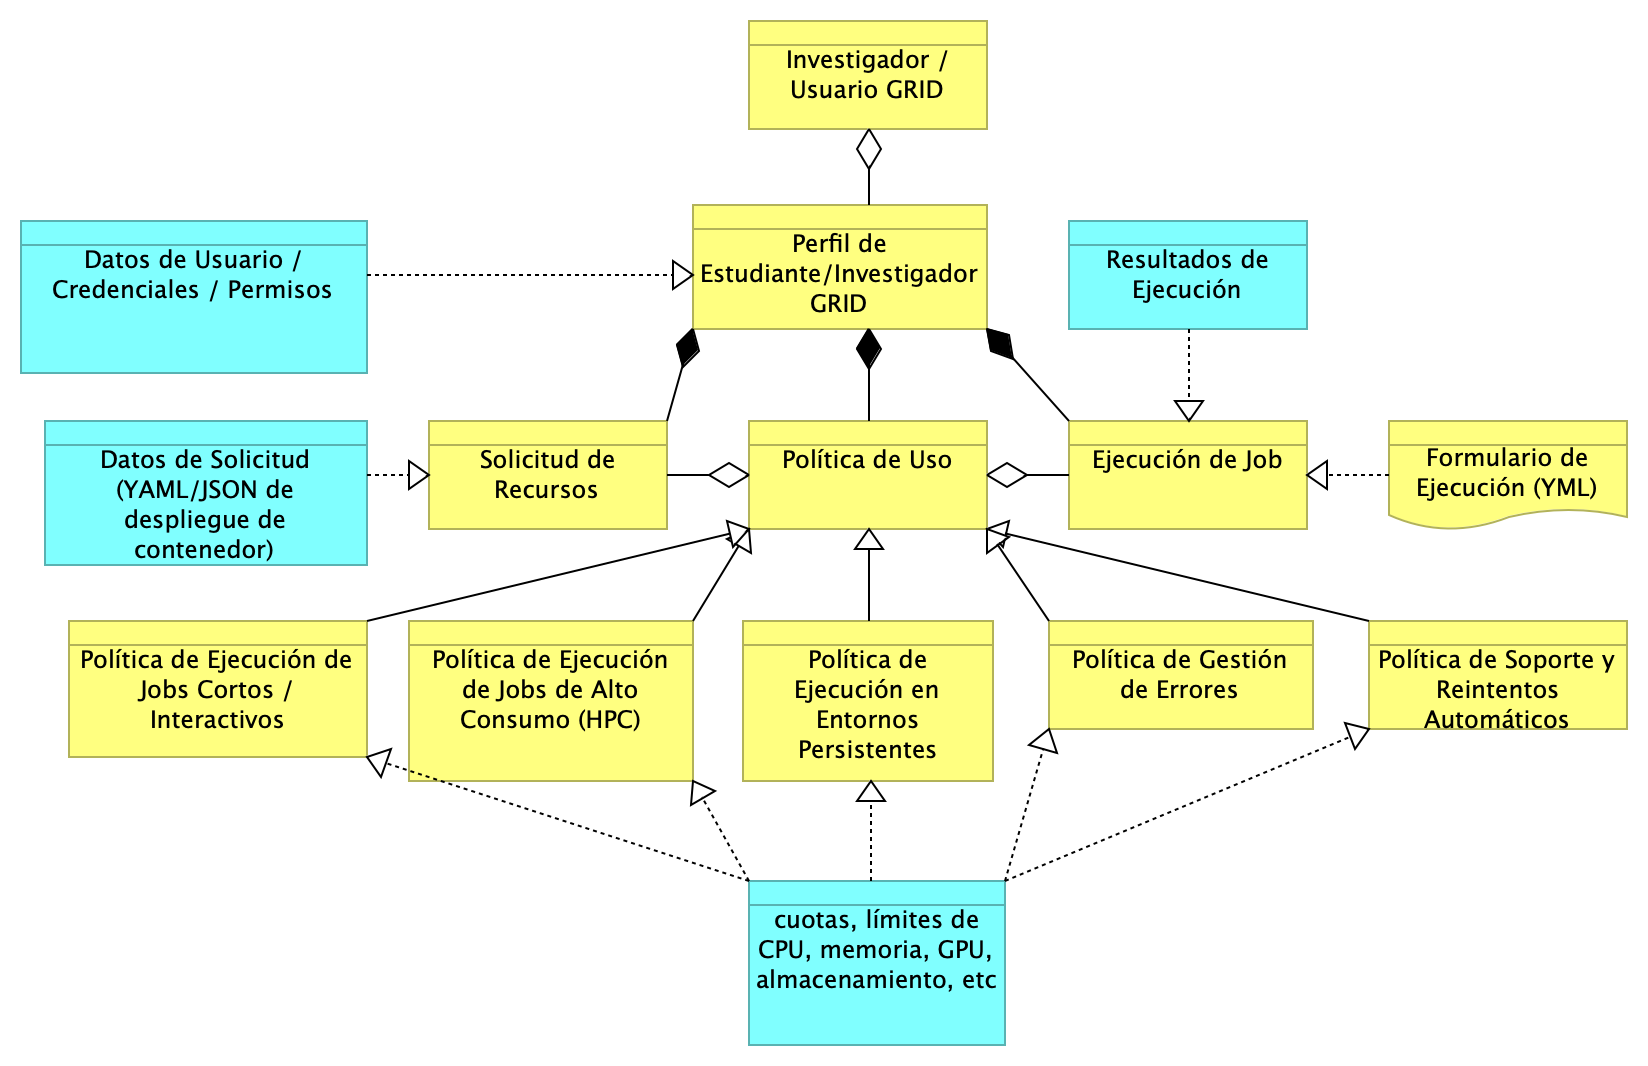
\includegraphics[width=\textwidth]{tablas-images/cp6/Information-Structure-View.png}
    \caption{Vista de Estructura de Información}
\end{figure}x


\subsection{Vista general}
%% Vista general - Placeholder
% Este archivo contiene la vista general del modelo ArchiMate

\begin{figure}[H]
	\centering
	
\includegraphics[width=\textwidth]{images/placeholder.png}
	\caption{Vista general del sistema}
	\label{fig:vista-general}
\end{figure}

% Descripción de la vista general
La vista general integra las tres capas del modelo ArchiMate (negocio, aplicación y tecnología) para proporcionar una perspectiva completa de la arquitectura de la solución. Esta vista permite visualizar las relaciones y dependencias entre los diferentes elementos del sistema HTCondor, desde los procesos de negocio hasta la infraestructura tecnológica que los soporta.

Esta vista consolidada facilita la comprensión del sistema en su totalidad y sirve como herramienta de comunicación entre los diferentes stakeholders del proyecto, permitiendo identificar puntos de integración críticos y oportunidades de optimización en toda la arquitectura.


\section{Diseño por capas de la solución}

\section{Capa de infraestructura}

\begin{figure}[H]
    \centering
    %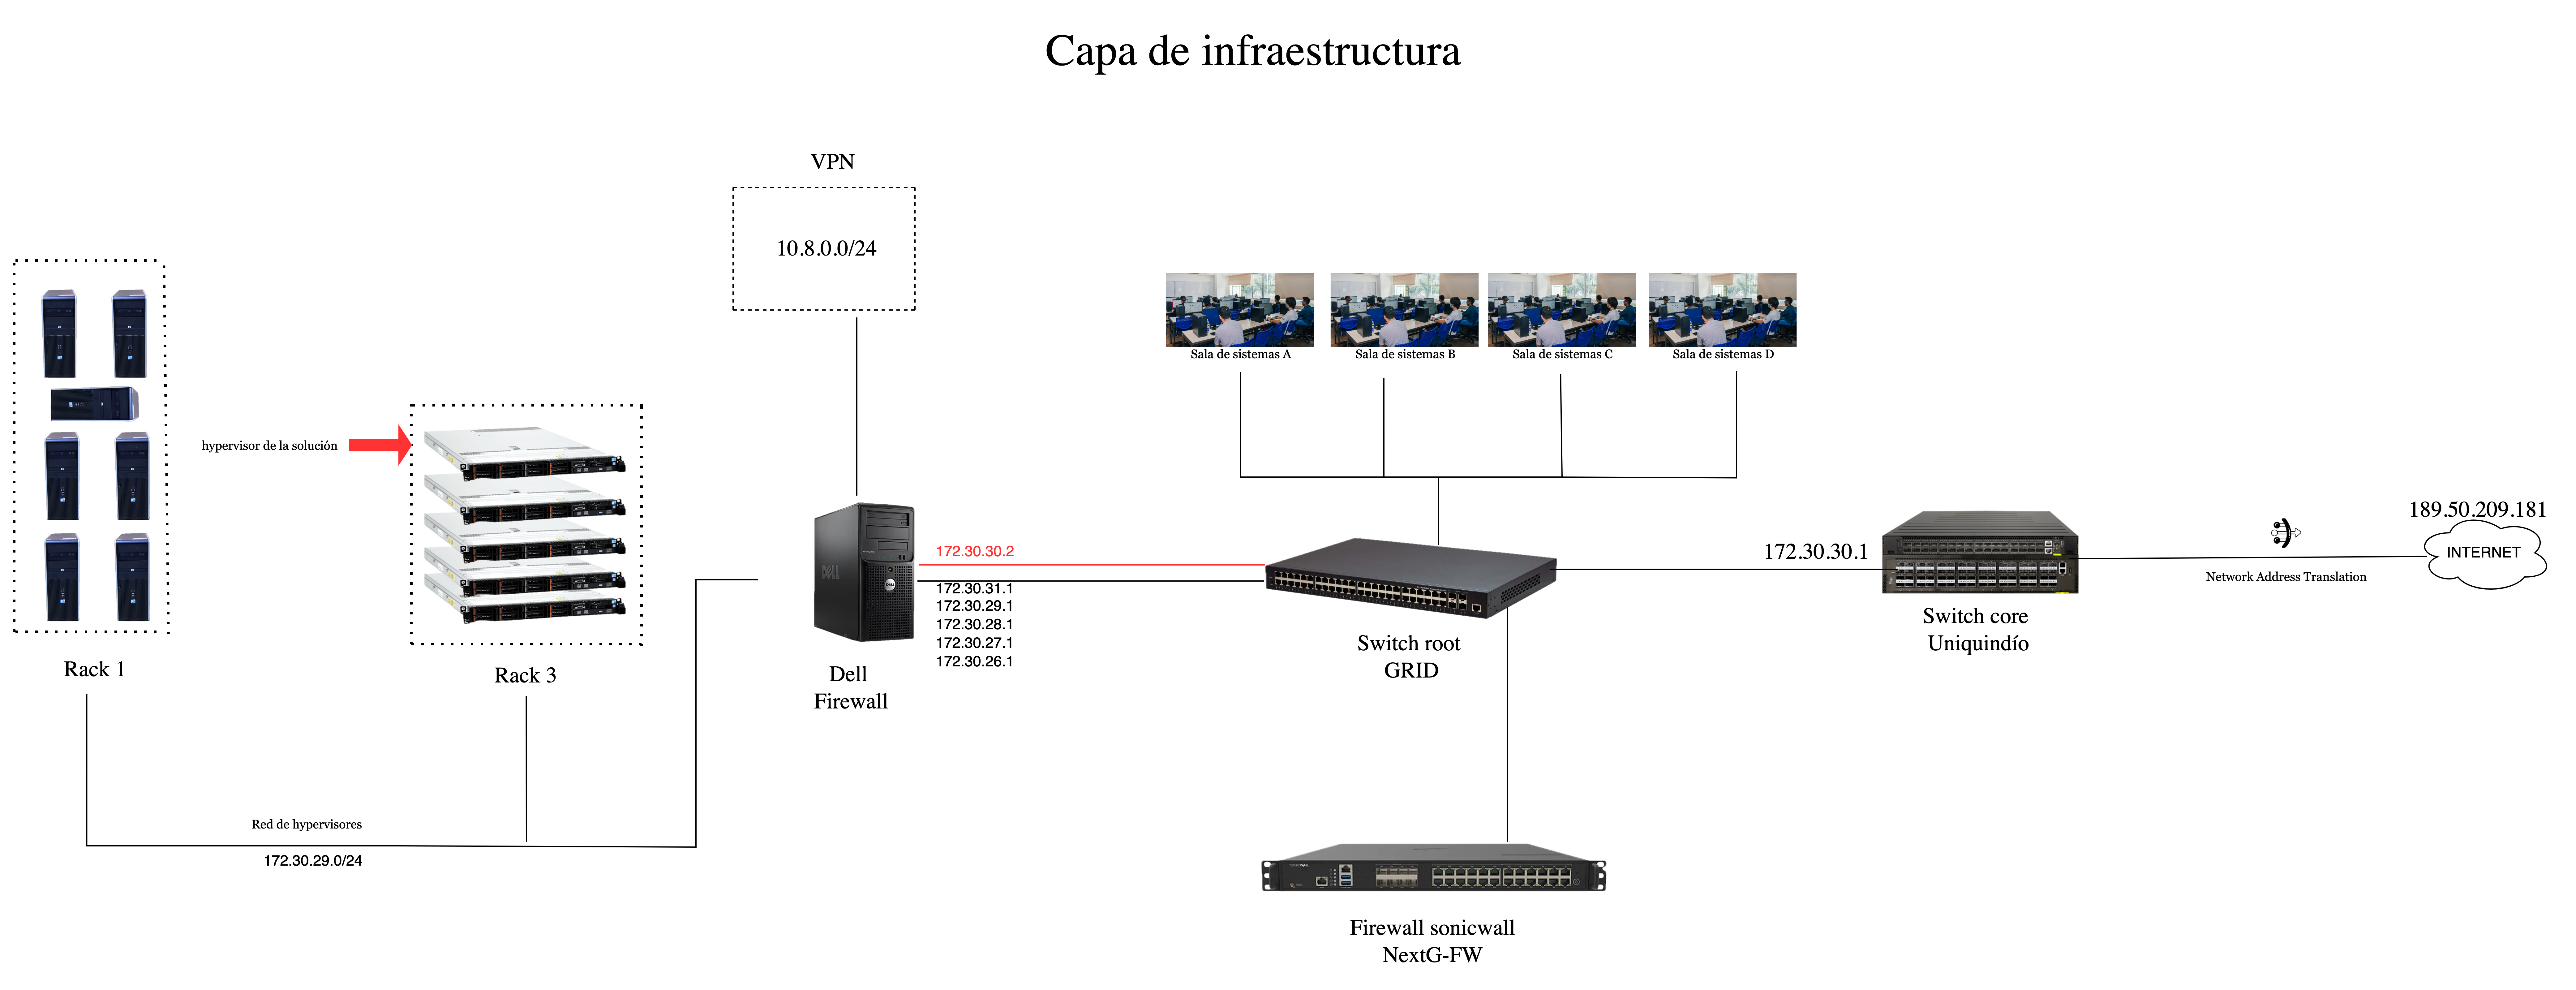
\includegraphics[width=\textwidth]{tablas-images/cp6/disenio-N1.png}
    \caption{Capa de Infraestructura}
\end{figure}

\section{Capa de virtualización}

\begin{figure}[H]
    \centering
    %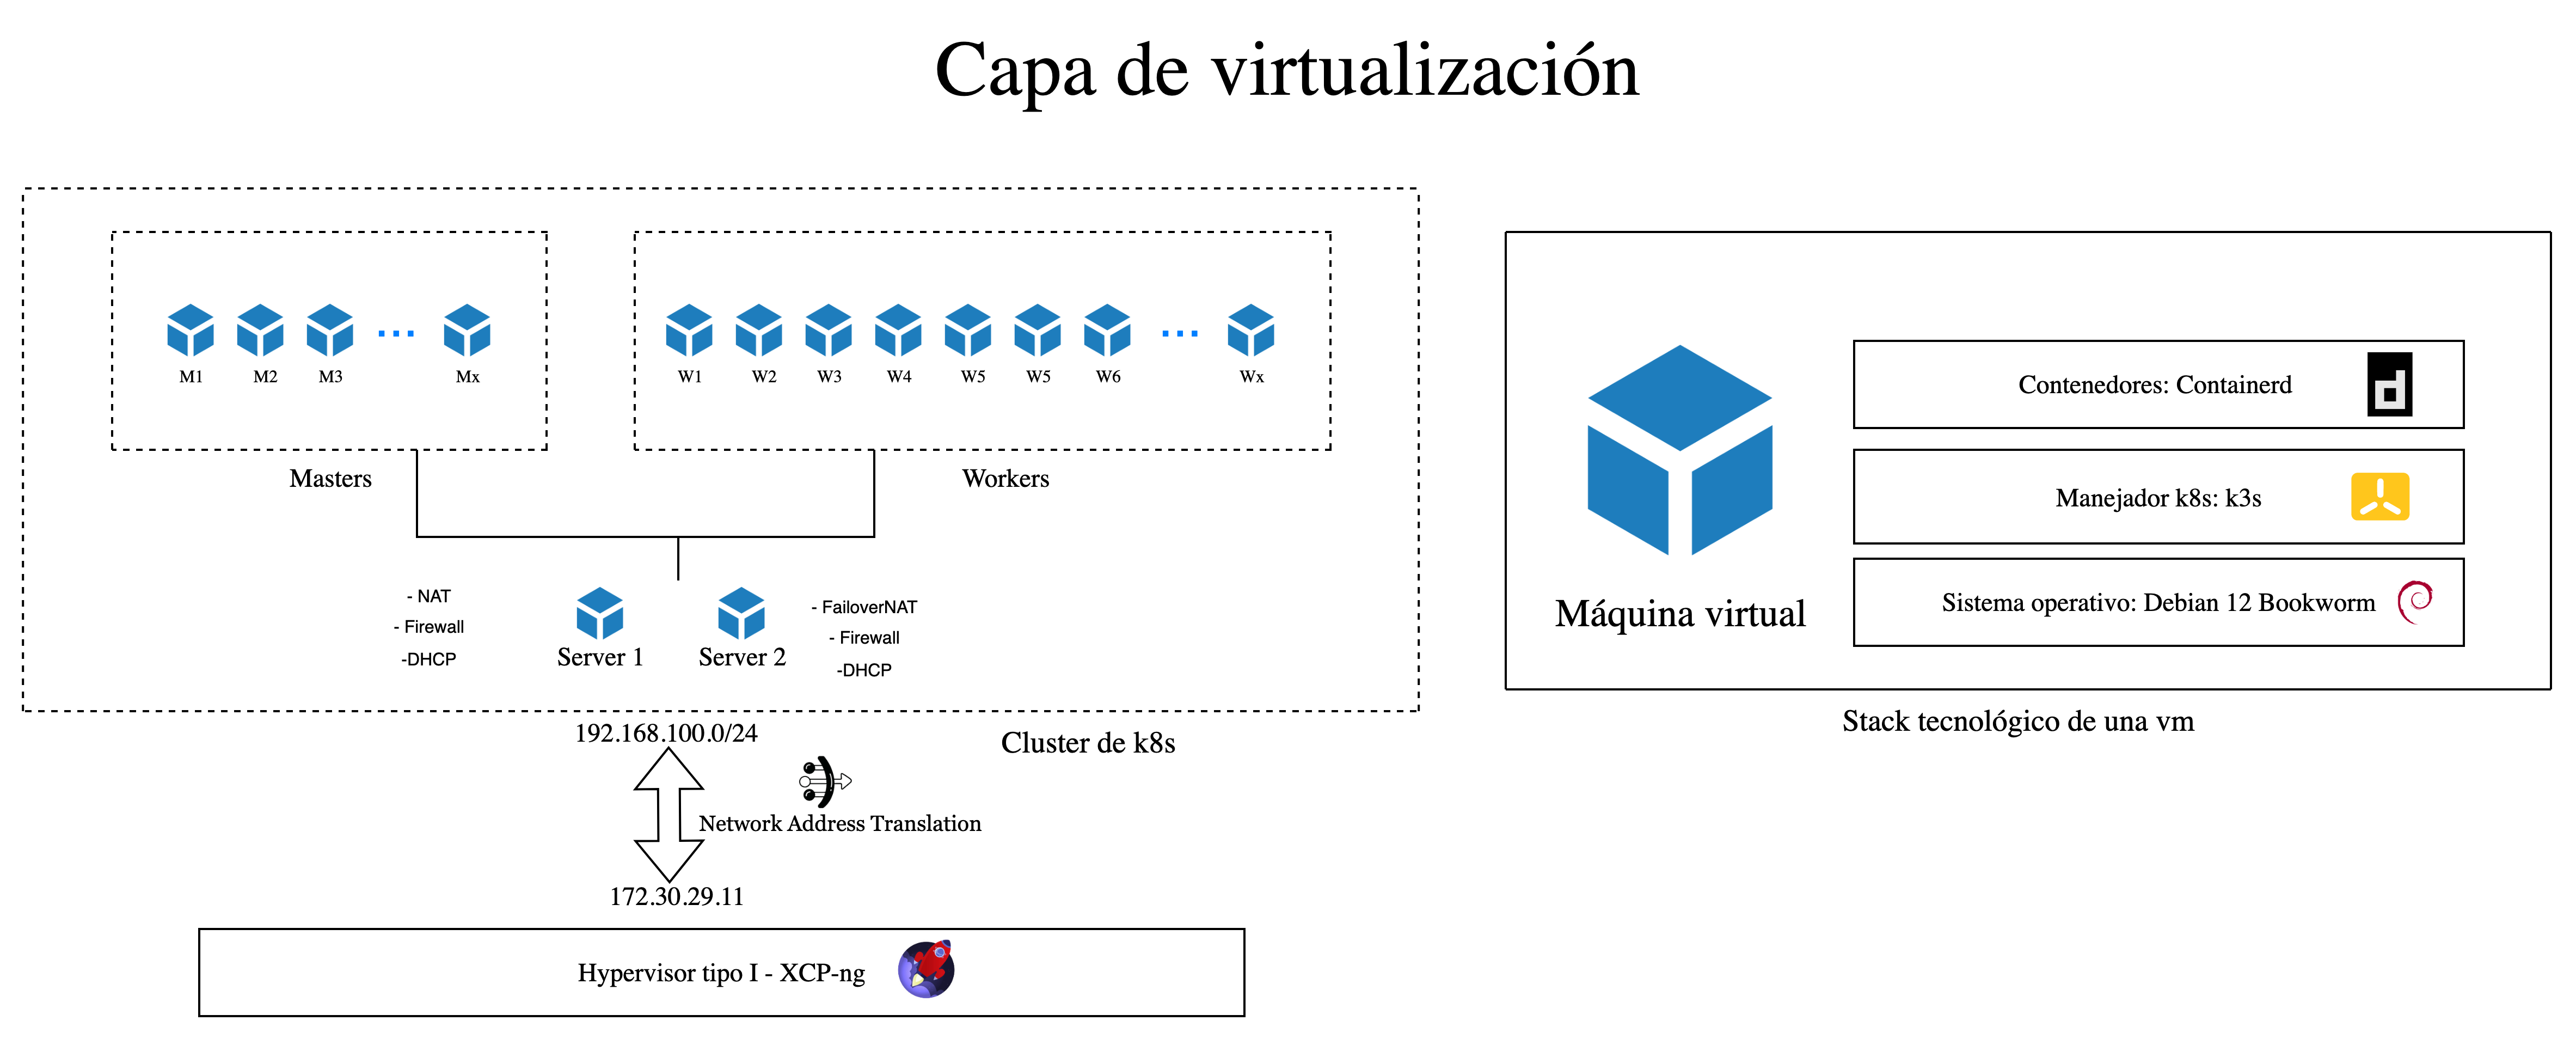
\includegraphics[width=\textwidth]{tablas-images/cp6/disenio-N2.png}
    \caption{Capa de Virtualización}
\end{figure}

\section{Capa de aplicación}
